\documentclass[tikz,border=8pt]{standalone}
\usepackage{amsmath}
\usetikzlibrary{arrows.meta,positioning,fit}

\begin{document}
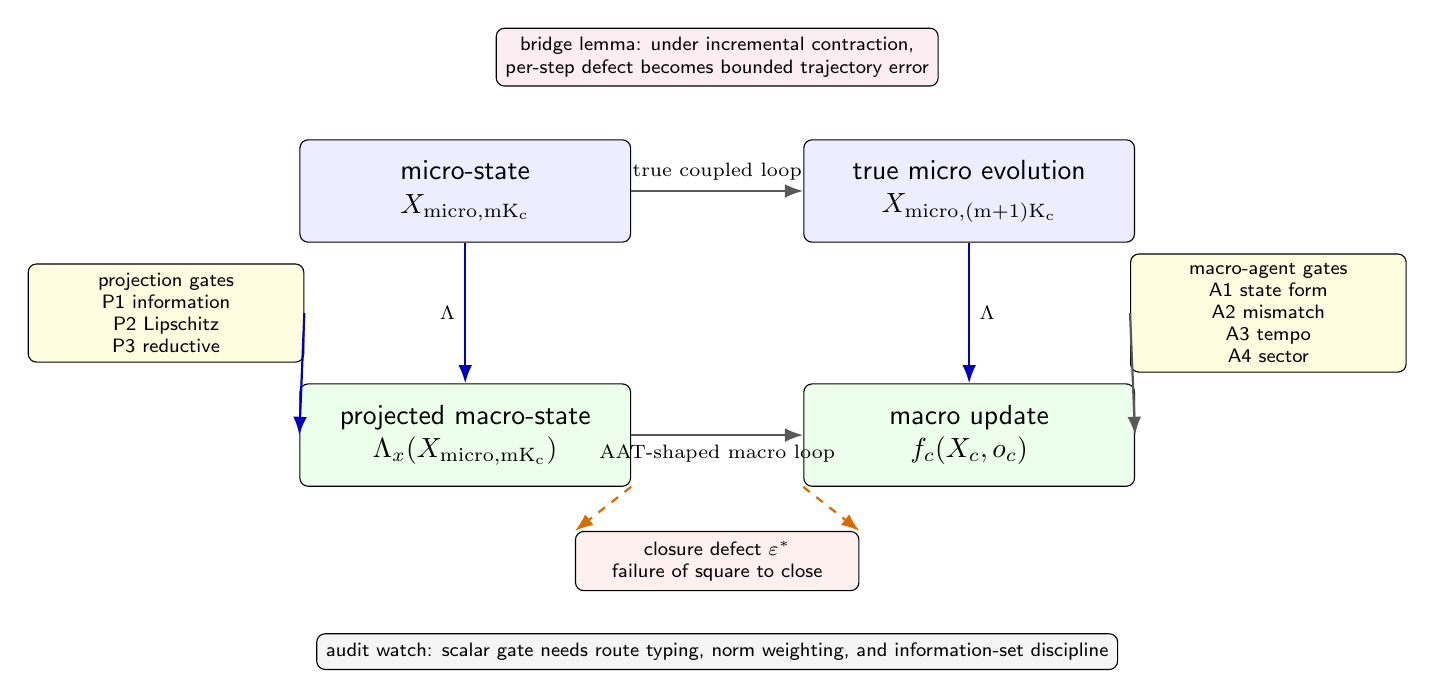
\begin{tikzpicture}[
  font=\sffamily,
  box/.style={draw, rounded corners=3pt, align=center, minimum width=42mm, minimum height=13mm, fill=white},
  gate/.style={draw, rounded corners=3pt, align=center, font=\sffamily\scriptsize, minimum width=35mm, minimum height=10mm, fill=yellow!12},
  note/.style={draw, rounded corners=3pt, align=center, font=\sffamily\scriptsize, fill=white},
  arrow/.style={-Latex, thick, draw=black!65},
  proj/.style={-Latex, thick, draw=blue!75!black},
  warn/.style={-Latex, thick, dashed, draw=orange!85!black}
]

\node[box, fill=blue!7] (micro0) at (-3.2,1.6)
  {micro-state\\$X_{\rm micro,mK_c}$};
\node[box, fill=blue!7] (micro1) at (3.2,1.6)
  {true micro evolution\\$X_{\rm micro,(m+1)K_c}$};
\node[box, fill=green!8] (macro0) at (-3.2,-1.5)
  {projected macro-state\\$\Lambda_x(X_{\rm micro,mK_c})$};
\node[box, fill=green!8] (macro1) at (3.2,-1.5)
  {macro update\\$f_c(X_c,o_c)$};

\draw[arrow] (micro0.east) -- node[above, font=\scriptsize] {true coupled loop} (micro1.west);
\draw[proj] (micro0.south) -- node[left, font=\scriptsize] {$\Lambda$} (macro0.north);
\draw[proj] (micro1.south) -- node[right, font=\scriptsize] {$\Lambda$} (macro1.north);
\draw[arrow] (macro0.east) -- node[below, font=\scriptsize] {AAT-shaped macro loop} (macro1.west);

\node[note, fill=red!6, minimum width=36mm] (eps) at (0,-3.1)
  {closure defect $\varepsilon^\ast$\\failure of square to close};
\draw[warn] (macro1.south west) -- (eps.north east);
\draw[warn] (macro0.south east) -- (eps.north west);

\node[gate] (pgate) at (-7.0,0.05)
  {projection gates\\P1 information\\P2 Lipschitz\\P3 reductive};
\node[gate] (agate) at (7.0,0.05)
  {macro-agent gates\\A1 state form\\A2 mismatch\\A3 tempo\\A4 sector};
\draw[proj] (pgate.east) -- (macro0.west);
\draw[arrow] (agate.west) -- (macro1.east);

\node[note, fill=purple!7, minimum width=52mm] (bridge) at (0,3.3)
  {bridge lemma: under incremental contraction,\\per-step defect becomes bounded trajectory error};
\node[note, fill=gray!8, minimum width=72mm] at (0,-4.25)
  {audit watch: scalar gate needs route typing, norm weighting, and information-set discipline};

\end{tikzpicture}
\end{document}
